% !TeX spellcheck = en_US
\chapter{Value Function Based Algorithms}
\section{Approach}
Knowing the value functions, we could just remove the policy gradient completely. The advantage function $A^\pi(\textbf{s}_t, \textbf{a}_t)$ tells how much better is $\textbf{a}_t$ than the average action according to policy $\pi$, regardless of what $\pi(\textbf{a}_t | \textbf{s}_t)$ is. We could have a policy $\pi'$ by simply choosing the current best action. $\pi'$ would be as good as $\pi$ (probably better).

\hlb{High-level idea for Policy Iteration:}
\begin{enumerate}
	\item \tikzmark{pi1}Evaluate $A^\pi(s,a)$ (policy evaluation)
	\item \tikzmark{pi2}Set $\pi \leftarrow \pi'$
	\begin{tikzpicture}[overlay,remember picture]
		\draw[very thick, -latex] ([xshift=-7mm,yshift=1mm]pic cs:pi2) --++ (-.5,0) |- ([xshift=-7mm,yshift=1mm]pic cs:pi1);
	\end{tikzpicture}
\end{enumerate}
\begin{equation}
	\pi'(\textbf{a}_t|\textbf{s}_t) = \begin{cases}
		1 \qquad \text{if } \textbf{a}_t = \underset{\textbf{a}_t}{\arg\max}\; A^\pi(\textbf{s}_t, \textbf{a}_t)\\
		0 \qquad \text{otherwise}
	\end{cases}
\end{equation}

\section{Policy Iteration with Dynamic Programming}
\hlb{Dynamic Programming}:
\begin{itemize}
	\item Assume we know $p(\textbf{s}'|\textbf{s,a})$
	\item $\textbf{s}$ and $\textbf{a}$ are both discrete and small
	\item $V^\pi(\textbf{s})$  can be stored in a lookup table
	\item $\mathcal{T}$ is a tensor
\end{itemize}

\hlb{Algorithm:}
\begin{enumerate}
	\item \tikzmark{pidp1}$V^\pi(\textbf{s}) \leftarrow r(\textbf{s}, \pi(\textbf{s})) + \gamma\mathbb{E}_{\textbf{s}'\sim p(\textbf{s}'|\textbf{s},\pi(\textbf{s}))} [V^\pi(\textbf{s}')]$
	\item \tikzmark{pidp2}Set $\pi \leftarrow \pi'$
	\begin{tikzpicture}[overlay,remember picture]
		\draw[very thick, -latex] ([xshift=-7mm,yshift=1mm]pic cs:pidp2) --++ (-.5,0) |- ([xshift=-7mm,yshift=1mm]pic cs:pidp1);
	\end{tikzpicture}
\end{enumerate}

\section{Value Iteration Algorithm}
\label{sec:value-iteration}
Since $\underset{\textbf{a}_t'}{\arg\max}\; A^\pi(\textbf{s}_t, \textbf{a}_t) = \underset{\textbf{a}_t'}{\arg\max}\; Q^\pi(\textbf{s}_t, \textbf{a}_t)$, we can simplify above \ac{algor}:
\begin{enumerate}
	\item \tikzmark{vi1}Set $Q^\pi(\textbf{s, a}) \leftarrow r(\textbf{s, a}) + \gamma\mathbb{E}[V^\pi(\textbf{s}')]$
	\item \tikzmark{vi2}Set $V^\pi(\textbf{s}) \leftarrow \underset{\textbf{a}}{\max}\; Q^\pi(\textbf{s, a})$
	\begin{tikzpicture}[overlay,remember picture]
		\draw[very thick, -latex] ([xshift=-7mm,yshift=1mm]pic cs:vi2) --++ (-.5,0) |- ([xshift=-7mm,yshift=1mm]pic cs:vi1);
	\end{tikzpicture}
\end{enumerate}

\section{Fitted Value Iteration}
The above two approaches still have a table to fit the value functions. For larger state space (either continuous or discrete), when facing the curse of dimensionality (for \textbf{$s$}), we shall use neural network to evaluate the value functions.
\begin{enumerate}
	\item \tikzmark{fvi1}$\textbf{y}_i \leftarrow \underset{\textbf{a}_i}{\max}\; r(\textbf{s}_i, \textbf{a}_i) + \gamma\mathbb{E}\left[ V_{\phi}(\textbf{s}_i') \right]$
	\item \tikzmark{fvi2}$\phi \leftarrow \underset{\phi}{\arg\min}\;\frac{1}{2} \sum_{i} ||V_{\phi}(\textbf{s}_i) - \textbf{y}_i||^2$
	\begin{tikzpicture}[overlay,remember picture]
		\draw[very thick, -latex]
		([xshift=-7mm,yshift=1mm]pic cs:fvi2) --++ (-.5,0) |-
		([xshift=-7mm,yshift=1mm]pic cs:fvi1);
	\end{tikzpicture}
\end{enumerate}
\begin{figure}[hbt!]	
	\centering
	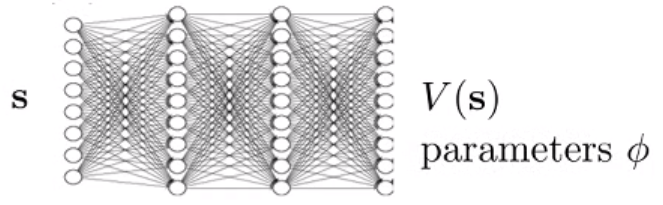
\includegraphics[width=.5\textwidth]{fitted-value-iteration.png}
	\caption{The network for value function $V_{\phi}(s)$ with \ac{param} $\phi$.}
	\label{fig:fitted-value-iteration}
\end{figure}
\hlb{Problem:} still need to know transition dynamic.

\section{Fully fitted Q-Iteration}
Policy evaluation:
\begin{itemize}
	\item $V^\pi(\textbf{s}) \leftarrow r(\textbf{s}, \pi(\textbf{s})) + \gamma\mathbb{E}_{\textbf{s}'\sim p(\textbf{s}'|\textbf{s},\pi(\textbf{s}))} [V^\pi(\textbf{s}')]$ needs to know the transition models
	\item $Q^\pi(\textbf{s, a}) \leftarrow r(\textbf{s, a}) + \gamma\mathbb{E}_{\textbf{s}'\sim p(\textbf{s}'|\textbf{s, a})} [Q^\pi(\textbf{s}', \pi(\textbf{s}'))]$ needs only a sample tuple $\{\textbf{s, a, s}'\}$
\end{itemize}
Replacing since $\mathbb{E}[V(\textbf{s}_i')] \approx \underset{\textbf{a}'}{\max}\; Q_\phi(\textbf{s}_i', \textbf{a}_i')$ into fitted value iteration algorithm, we have Fully fitted Q-iteration:\\
{
	1. \tikzmark{ffqi1}Collect dataset: $\{(\textbf{s}_i, \textbf{a}_i, \textbf{s}_i', r_i)\}$ using some policy\\
	\tab 2. \tikzmark{ffqi2}Set $\textbf{y}_i \leftarrow r(\textbf{s}_i, \textbf{a}_i) + \gamma \underset{\textbf{a}_i'}{\max}\; Q_\phi (\textbf{s}_i', \textbf{a}_i')$\\
	\tab 3. \tikzmark{ffqi3}Set $\phi \leftarrow \underset{\phi}{\arg\min}\; \frac{1}{2} \sum_{i} || Q_{\phi}(\textbf{s}_i, \textbf{a}_i) - \textbf{y}_i ||^2$
	\begin{tikzpicture}[overlay,remember picture]
		\draw[very thick, -latex]
		([xshift=-7mm,yshift=1mm]pic cs:ffqi3) --++ (-.5,0) |-
		([xshift=-7mm,yshift=1mm]pic cs:ffqi2);
		\draw[very thick, -latex]
		([xshift=-7mm,yshift=0mm]pic cs:ffqi3) --++ (-1.2,0) |-
		([xshift=-5mm,yshift=1mm]pic cs:ffqi1);
		\node at ([xshift=-14mm,yshift=7mm]pic cs:ffqi3) {\fontsize{10}{0}\selectfont \rotatebox{90}{$K \times$}};
	\end{tikzpicture}
}

\begin{figure}[hbt!]
	\centering
	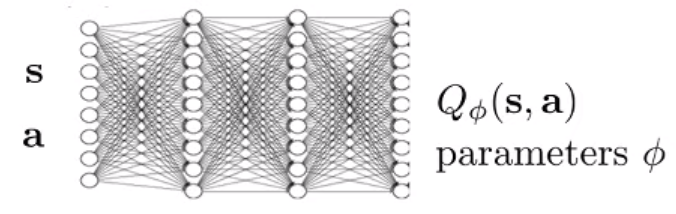
\includegraphics[width=.5\textwidth]{fully-fitted-q-iteration.png}
	\caption{The network for Q-value function $Q_{\phi}(s,a)$ with \ac{param} $\phi$.}
	\label{fig:fully-fitted-q-iteration}
\end{figure}
$\begin{matrix*}[l]
	\color{Green}+ \text{Off-policy (unlike actor-critic)}\\
	\color{Green}+\text{Single network, no high-variance policy gradient}\\
	\color{red}- \text{Not really converge}
\end{matrix*}$

\section{Online Q-Iteration Algorithm}
\begin{enumerate}
	\item \tikzmark{oqi1}Take some action $\textbf{a}_i$ and observe $(\textbf{s}_i, \textbf{a}_i, \textbf{s}_i', r_i)$ \qquad\hlr{1 sample off policy}
	\item $\textbf{y}_i \leftarrow r(\textbf{s}_i, \textbf{a}_i) + \gamma\underset{\textbf{a}_i'}{\max}\; Q_\phi(\textbf{s}_i', \textbf{a}_i')$
	\item \tikzmark{oqi3}$\displaystyle\phi \leftarrow \phi - \alpha\frac{dQ_\phi}{d\phi}(\textbf{s}_i, \textbf{a}_i)\left[ Q_\phi(\textbf{s}_i, \textbf{a}_i) - \textbf{y}_i \right]$  \qquad\qquad\hlr{1 gradient step}
	\begin{tikzpicture}[overlay,remember picture]
		\draw[very thick, -latex]
		([xshift=-7mm,yshift=1mm]pic cs:oqi3) --++ (-.5,0) |-
		([xshift=-7mm,yshift=1mm]pic cs:oqi1);
	\end{tikzpicture}
\end{enumerate}
\hlb{Problems:}
\begin{itemize}
	\item Sequential states are strongly correlated $\Rightarrow$ Replay buffer
	\item Target value is always changing $\Rightarrow$ Target network
\end{itemize}

\section{Exploration vs Exploitation}
\begin{itemize}
	\item Epsilon greedy
	\begin{equation}
		\pi(\textbf{a}_t|\textbf{s}_t) = \begin{cases}
			1-\epsilon \quad\qquad \text{if } \textbf{a}_t = \underset{\textbf{a}_t}{\arg\max}\; A^\pi(\textbf{s}_t, \textbf{a}_t)\\
			\displaystyle \frac{\epsilon }{|\mathcal{A}|-1} \qquad \text{otherwise}
		\end{cases}
	\end{equation}
	\item Boltzmann exploration \hlr{(very large or continuous action-space)}
	\begin{equation}
		\pi(\textbf{a}_t | \textbf{s}_t) \propto \exp (Q_\phi(\textbf{s}_t, \textbf{a}_t))
	\end{equation}
\end{itemize}

\section{Q-learning}
Q-learning with replay buffer $\mathcal{B}$ and target network $\phi'$:\\
{1. \tikzmark{ql1}Save target network \ac{param} $\phi' \leftarrow \phi$\\
	\tab 2. \tikzmark{ql2}Collect dataset $\{(\textbf{s}_i, \textbf{a}_i, \textbf{s}_i', r_i) \}$ using some policy, add it to $\mathcal{B}$\\
	\tab\tab 3. \tikzmark{ql3}Sample a batch $(\textbf{s}_i, \textbf{a}_i, \textbf{s}_i', r_i)$ from $\mathcal{B}$\\
	\tab\tab 4. \tikzmark{ql4}$\displaystyle\phi \leftarrow \phi - \alpha\sum_{i} \frac{dQ_\phi}{d\phi}(\textbf{s}_i, \textbf{a}_i)\left( Q_\phi(\textbf{s}_i, \textbf{a}_i) - \left[ r(\textbf{s}_i, \textbf{a}_i) + \gamma\underset{a'}{\max}\; Q_{\phi'}(\textbf{s}_i', \textbf{a}_i') \right]\right)$\\
	$K \in [1, 4], N \approx 10,000$
	\begin{tikzpicture}[overlay,remember picture]
		\draw[very thick, -latex]
		([xshift=-7mm,yshift=2mm]pic cs:ql4) --++ (-.5,0) |-
		([xshift=-7mm,yshift=1mm]pic cs:ql3);
		\draw[very thick, -latex]
		([xshift=-7mm,yshift=1mm]pic cs:ql4) --++ (-1.2,0) |-
		([xshift=-5mm,yshift=1mm]pic cs:ql2);
		\draw[very thick, -latex]
		([xshift=-7mm,yshift=0mm]pic cs:ql4) --++ (-2.2,0) |-
		([xshift=-5mm,yshift=1mm]pic cs:ql1);
		\node at ([xshift=-14mm,yshift=5mm]pic cs:ql4) {\fontsize{10}{0}\selectfont \rotatebox{90}{$K \times$}};
		\node at ([xshift=-22mm,yshift=2mm]pic cs:ql3) {\fontsize{10}{0}\selectfont \rotatebox{90}{$N \times$}};
\end{tikzpicture}}

\section{Deep Q-learning}
\label{sec:dql}
\begin{enumerate}
	\item \tikzmark{dql1}Take some action $\textbf{a}_i$ and observe $(\textbf{s}_i, \textbf{a}_i, \textbf{s}_i', r_i)$, add it to $\mathcal{B}$
	\item Sample mini-batch $\{(\textbf{s}_j, \textbf{a}_j, \textbf{s}_j', r_j) \}$ from $\mathcal{B}$ uniformly
	\item Compute $y_j = r_j + \gamma \underset{\textbf{a}_j'}{\max} Q_{\phi'}(\textbf{s}_j', \textbf{a}_j')$ using \textit{target} network $Q_{\phi'}$
	\item $\phi \leftarrow \phi - \alpha \sum_j \frac{dQ_\phi}{d\phi}(\textbf{s}_j, \textbf{a}_j) \left( Q_{\phi}(\textbf{s}_j, \textbf{a}_j) - y_j \right)$
	\item \tikzmark{dql5}Update $\phi'$: copy $\phi$ every $N$ steps
	\begin{tikzpicture}[overlay,remember picture]
		\draw[very thick, -latex]
		([xshift=-7mm,yshift=1mm]pic cs:dql5) --++ (-.5,0) |-
		([xshift=-7mm,yshift=1mm]pic cs:dql1);
	\end{tikzpicture}
\end{enumerate}
The above \textit{"Classic"} \ac{DQN} is essentially Q-learning with $K=1$ \cite{mnih2015human}

Improving \ac{DQN}:
\begin{itemize}
	\item Alternative: Step 5. Update $\phi' \leftarrow \tau\phi' + (1-\tau)\phi, \quad \tau = 0.999$ (Polyak averaging)
	\item Double Q-learning: \hlr{helps a lot, solve over-estimate problem, no downside}\\
	\hlr{$\Rightarrow$ should always use}
	\begin{align}
		&\text{Standard Q-learning:} && y = r + \gamma Q_{\phi'}\left( s', \underset{a'}{\arg\max} Q_{\color{red} \phi'}(s', a') \right)\\
		&\text{Double Q-learning:} && y = r + \gamma Q_{\phi'}\left( s', \underset{a'}{\arg\max} Q_{\color{red} \phi}(s', a') \right)
	\end{align}
	\item Multi-Step returns: \hlr{helps a lot, have DOWNSIDE $\Rightarrow$ frequently use} \cite{munos2016safe}
	\begin{align}
		& \text{Q-learning target:} && y_{i,t} = r_{i,t} + \gamma\; \underset{a_{i, t+1}}{\max} Q_{\phi'}(\textbf{s}_{i, t+1}, a_{i, t+1})\\
		& \text{Multi-step target:} && y_{i,t} = \sum_{t'=t}^{t+N-1} \gamma^{t'-t} r_{i,t'} + \gamma^N \underset{a_{i, t+N}}{\max} Q_{\phi'}(\textbf{s}_{i, t+N}, a_{i, t+N})
	\end{align}
	$\begin{matrix*}[l]
		\color{Green} + \text{less biased target values when Q-values are inaccurate}\\
		\color{Green} + \text{typically faster learning, especially early on}\\
		\color{red} - \text{Only actually CORRECT when learning on-policy}
	\end{matrix*}$
\end{itemize}

\section{Q-learning with continuous action-space}
\todo{}

\section{Tips for Q-learning}
\begin{itemize}
	\item Large replay buffer helps improve stability (1 Million).
	\item Apply Prioritized Experience Replay \cite{schaul2015prioritized}
	\item It takes time, be patient - might be no better than random for a while
	\item Start with high exploration $\Rightarrow$ gradually reduce
	\item Bellman error gradient can be quite large $\Rightarrow$ clip gradients / use Huber loss
	\begin{equation}
		L(x) = \begin{cases}
			\frac{x^2}{2} \quad \text{if } |x| \leq \delta\\
			\delta|x| - \frac{\delta^2}{2} \quad \text{otherwise}
		\end{cases} \qquad \text{(Huber loss)}
	\end{equation}
	\item Run multiple random seeds, it's very \hlb{inconsistent} between runs.	
\end{itemize}

\section{Policy Gradient as Policy Iteration}
\todo{math stuffs}

\section{References}
\begin{itemize}
	\item \citeaustitle{watkins1989learning}
	\item \citeaustitle{riedmiller2005neural}
	\item \citeaustitle{lange2010deep}
	\item \citeaustitle{mnih2015human}
	\item \citeaustitle{van2016deep}
	\item \citeaustitle{lillicrap2015continuous}
	\item \citeaustitle{gu2016continuous}
	\item \citeaustitle{wang2016dueling}
	\item \citeaustitle{kalashnikov2018qt}
\end{itemize}